\section{Network architecture}

Numerous architectural designs have been developed in the literature for the MNIST dataset, given its role as a benchmark in image classification. These architectures varies in both complexity and the level of attained accuracy. To understand the task in a better way, a standard architecture will be introduced as a point of reference. Subsequently, the architecture employed in this study will be presented.

\subsection{Reference architecture}

The reference architecture utilized for the MNIST dataset is the one presented in the research conducted by Le Cun et al. \cite{LeCun:90}, known as \textit{LeNet-5}. This network is a CNN and it is organized into two principal components:

\begin{itemize}
	\item The initial segment consists in two convolutional layers coupled with pooling, interpretable as the component accountable for feature extraction.;
	\item The subsequent section includes three fully connected layers, assuming the role of classification by exploiting the features previously extracted.
\end{itemize}

The graphical representation of the LeNet-5 architecture is provided in \Fig~\ref{fig:lenet5}.

\begin{figure}[h]
	\centering
	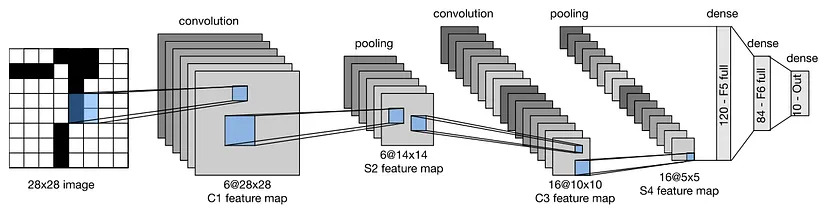
\includegraphics[width=0.8\linewidth]{ImageFiles/NetArchitecture/lenet5}
	\caption{LeNet-5 architecture \cite{LeNet5}}
	\label{fig:lenet5}
\end{figure}

During the experimentation detailed in \cite{LeCun:90}, the network was trained utilizing the MSE as loss function, with 30 epochs. This training yielded to an accuracy of 98.9\% when applied to the training set, and a slightly lower accuracy of 96.6\% when evaluated on the test set. These numerical values will serve as benchmark metrics for the comparison.

\subsection{Proposed architecture}

Although for image processing tasks CNNs are typically considered a more advantageous choice, for this case study, a MLP has been chosen as network type. The reason behind this decision is the more understandable and intuitive MLP structure, which is well-suited to the main objective of this work.

CNNs rely on convolutional layers, which utilize a mathematical operation known as convolution. The learnable parameters in convolutional layer are the values of the kernel functions applied. Nevertheless, during the design phase, CNNs involve more hyperparameters to specify, such as the number of filters, their dimensions, stride, and padding. While this enhances CNNs effectiveness when dealing with grid-scale data, it simultaneously adds complexity to the model interpretation. In contrast, MLPs offer a more straightforward structure, as every neuron connects with all others, and the modifiable parameters consist of the connection weights.

Since the primary focus here is not on image classification, but rather on the investigation of the Bayesian approach to NNs. Therefore, the simplicity and transparency of the MLP make it a suitable choice.

In this thesis, the term standard NN will denote an MLP that does not employ Bayesian inference.

In this study two NNs were developed: one standard and Bayesian. To ensure fair comparison, both networks have the same architecture. Each model consists of three \textit{Linear} layers, representing fully connected layers:

\begin{enumerate}
	\item Input layer: Composed by 784 neurons, corresponding to the input data size;
	\item Hidden layer: This layer contains 100 neurons;
	\item Output layer: Consisting of 10 neurons, representing the number of classes to predict.
\end{enumerate}

The activation function used for the input and hidden layers is ReLU, while the output layer is activated using the softmax function. This enforces obtaining values between 0 and 1, which can be interpreted as probabilities.